\section{Graduate Students Perception}
\label{sec:students:perception}

The \texttt{OpenMP} exercise was proposed just after basic concepts of parallelism with shared memory were taught to the students.
The wording of the exercise was: \emph{\lq\lq{}Search for a sample code in \texttt{OpenMP} tutorials and manuals on the Internet that uses compilation directives and has some kind of error. Write a report introducing the code, pointing the problems and describing which are the corrections made to eliminate error.\rq\rq{}}.

After that we provided an anonymous questionnaire using \emph{Google Forms}. The question was: \emph{\lq\lq{}What is your opinion about your \texttt{OpenMP} experience and the \texttt{OpenMP} exercise?\lq\lq{}}. We got 24 answers, all of them with positive feedback, and selected some of them below.

Several students commented on how easy it was to use \texttt{OpenMP}: \lq\lq{}... I appreciate the idea of annotating an already existing program...\rq\rq{}; \lq\lq{}... with \texttt{OpenMP} it is possible to make an application parallel with low effort.\rq\rq{}; \lq\lq{}Why, when I learned concurrent programming, I did not learn it (\texttt{OpenMP})?\rq\rq{}. The students appreciated learning and using \texttt{OpenMP} in a simple example.

Several students also commented on the lack of a more explicit vision: \lq\lq.{}..When we use threads explicitly, I have the impression that it is easier to understand possible problems.\rq\rq{}; \lq\lq{}When I use \texttt{OpenMP}, I am always afraid about the correctness, and if I used the correct optimization flags\rq\rq{}. There were also some complaints about how barriers work in \texttt{OpenMP}: \lq\lq{}I had little experience with \texttt{OpenMP} and \texttt{pthreads}, but I believe that the understanding of \texttt{pthreads} is easier for those who already have experience in C. The (\texttt{OpenMP}) implicit barriers make me confused, since I never know when there is or not a barrier.\rq\rq{}.

There were also some more interesting ideas: "This experience encouraged me to write programs easier to parallelize with \texttt{OpenMP}.".
The following answer summarizes the opinions on the ease of use of the API, and also on the possible difficulty of working with \texttt{OpenMP}: \lq\lq{}... \texttt{OpenMP} appears to be a good framework for productivity, that is, it allows the creation of concurrent programs in less time and with less code rather than with \texttt{pthreads}. But it does not make parallel programming a trivial or error-free task.\rq\rq{}.

In another question we asked the students about their experience with programming and about the difficulties they had learning \texttt{OpenMP} directives. Figure~\ref{fig:DifOpenMP} shows the results.

Many students reported that they had difficulties to learn \texttt{OpenMP}. The majority had no previous experience, as shown in Figure~\ref{fig:students:experience}. In Figure~\ref{fig:DifOpenMP} it can be seen that most students also had less than ten years of programming experience. There was only $31$ days between the \texttt{OpenMP} introductory classes and the due date of the assignment, and this may have contributed to their difficulties.

These answers provide some evidence that, despite being considered an easy approach, \texttt{OpenMP} also requires knowledge and experience.

\begin{figure}[ht]
\centering
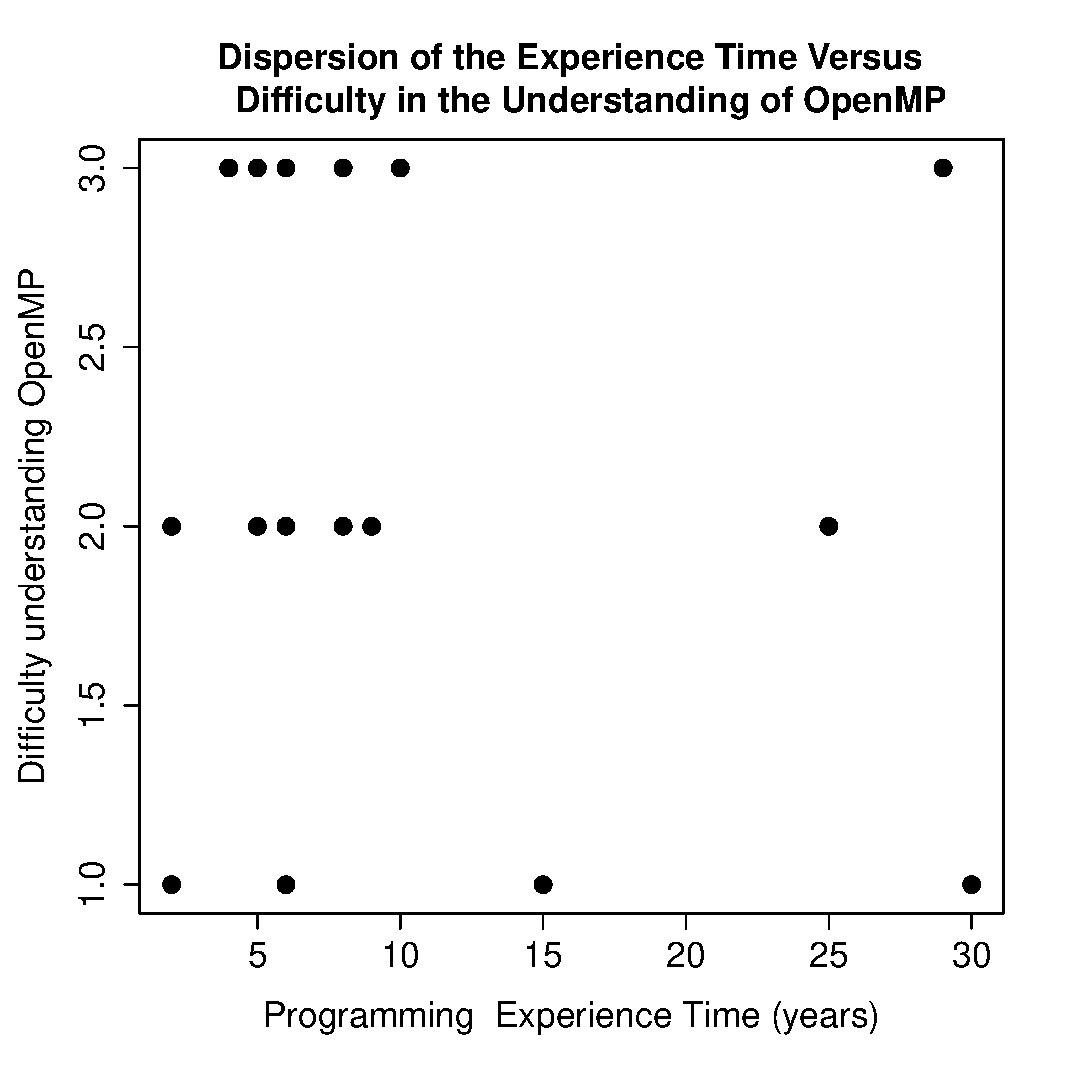
\includegraphics[width=0.95\columnwidth,height=0.9\columnwidth]{figures/experience.eps}
\caption{Graphic of dispersion of the experience time versus
    difficulty in the understanding of OpenMP}
\label{fig:DifOpenMP}
\end{figure}



\begin{comment}
Talvez seja importante falar também que os alunos tiveram aulas sobre conceitos de paralelismo antes.

Qual opinião você pode dar sobre sua experiência com \texttt{OpenMP} e sobre o Exercício de Programação 1?

1. Legal.

2. Achei interessante a ideia de anotar um programa que já funciona sequencialmente, mas esse método dificulta um pouco pensar em paralelo. Quando implementamos explicitamente as threads, tenho a impressão de que fica mais fácil entender os possíveis problemas.

3. Não conhecia o \texttt{OpenMP}, aparentemente é uma boa ferramenta, com alguma facilidade de aprendizado e já tenho utilizado para processamento de dados GPS sem maiores dificuldades. Sobre o EP1, aparentemente não trouxe grandes problemas técnicos. Apenas acho que, para efeito de aprendizado, ao invés de utilizar um grande problema, fosse mais conveniente propor mais pequenos problemas que servissem para salientar tópicos específicos.

4. Gostei bastante do EP1 por que o foco estava mais na compreensão de paralelismo e concorrência e menos num algoritmo complexo. Testes de desempenho sempre são divertidos e interessantes (comparação, interpretação).

5. Acredito que o EP1 foi bastante útil para o aprendizado das API do \texttt{OpenMP} para a utilização na prática.

6. Foi uma experiência interessante. Nunca tinha usado uma API de alto nivel. Só tinha usado semáforos e mutex. Gostei o fato que o \texttt{OpenMP} faz que, com pouco esforço, uma aplicação se torne paralela.

7. A implementação foi bem fácil (porque o problema era bem simples) e deu espaço para experimentarmos um pouco com as comparações e gráficos dos resultados; funcionou muito bem.

8. A utilização do \texttt{OpenMP} é bastante simples comparada com o uso de threads ou troca de mensagens como MPI (as duas outras ferramentas para programação paralela que eu tinha experiência anteriormente). Porém, os mesmos cuidados com deadlocks, granularidade, barreiras e etc. valem para o \texttt{OpenMP} também.

9. Foi instrutivo utilizar o \texttt{OpenMP}, apredner um outro método de fazer paralelismo

10. Enquanto estudava \texttt{OpenMP} fiquei pensando "por que raios isso não foi visto depois de pthread em Concorrente?".

11. Os exercícios foram simples de entender e nos permitiram avaliar a razão dos resultados obtidos.

12. Achei legal a experiência de ver a comparação de desempenho por processador e por número de threads. Outra coisa que gosto é a parte de focar mais no conceito e seu entendimento. EP simples que tocava exatamente no conceito me parece melhor que um EP super trabalhoso que talvez desse trabalho em pontos não relevantes à disciplina.

13. Quanto à \texttt{OpenMP} as dificuldades são relacionadas a: - corretude: será que nenhum caso foi esquecido (algo comum em paralelismo)? - otimização: será que a escolha foi a melhor possível para a implementação?
Quanto ao EP1, as dificuldades foram:
A maior dificuldade foi no exercício 1. Foi difícil definir uma estratégia para avaliar os códigos encontrados: compilar e executá-los poderia trazer problemas mais rápidos mas tomaria mais tempo um por um enquanto que avaliar somente analisando o código era mais difícil encontrar erros em um dado exemplo mas era possível analisar mais códigos. Quanto ao exercício 2, a dificuldade foi encontrar máquinas com arquiteturas diferentes. A menos que vc esteja envolvido em alguma área de computação científica ou paralela, a grande maioria dos computadores são x86.

14. Foi uma experiência positiva. Uma boa introdução a paralelização, que mostrou o quanto é prático usar \texttt{OpenMP}, pelo menos para uma aplicação simples como a do EP1. O problema em questão era suficientemente interessante para pensar nas questões do paralelismo por permitir várias formas de abordagem, e as ferramentas básicas do \texttt{OpenMP} foram suficientes para os experimentos e discussões.

15. Essa experiência me encorajou a usar o \texttt{OpenMP} em programas que eu venha a escrever e que sejam fáceis de paralelizar."

16. Tive contanto com conceitos de paralelismo no meu curso de graduação inclusive utilizando o \texttt{OpenMP}, porém a experiência da utilização do \texttt{OpenMP} neste trabalho foi muito melhor. Acho que senti bastantante a diferença neste EP1 por partirmos de uma versão sequencial, diferentemento do trabalho que fiz na graduação e o \texttt{OpenMP} se mostrou muito bem nesta situação.

17. O \texttt{OpenMP} é muito fácil de aprender mas há códigos com erros na internet, geralmente esses códigos tinham erros na operação "cout" do c++, geralmente usam ele para mostrar dados dentro de uma região paralela, pareceria que não sabem que essa operação não é atómica, outros tipos de erros que achei foram erros no código, por exemplo o erro mais comum que eu vi foram que eles não verificam se o indice de um arranjo é valido ou não; quer dizer que alguns tutoriais tem erros no mesmo algoritmo não verificam se o algoritmo é correcto ou não.

18. Foi o primeiro contato que tive com \texttt{OpenMP}. Achei bastante proveitoso aprender a utilizar o \texttt{OpenMP}. Além disso, foi divertido fazer experimentos para avaliar o desempenho do programa usando diferentes implementações.

19. O \texttt{OpenMP} me parece um bom framework para produtividade, ou seja, permite a criação de programas concorrentes em menos tempo e com menos código do que com pthreads, por exemplo, mas não torna a programação paralela uma tarefa trivial ou livre de erros.

20. "O \texttt{OpenMP} oferece uma sintaxe concisa para resolver um problema complexo. Dominar o poder que a interface proporciona requer um tempo considerável de estudo e reflexão para se chegar ao resultado esperado, portanto trata-se muito mais de um exercício intelectual do que mecânico.
A sintaxe tem uma carga conceitual muito grande. Tenho experiência em trabalhar com outras linguagens que têm características semelhantes de concisão e carga conceitual (por exemplo, Ruby) e acredito que leva um tempo relativamente mais alto para se obter proficiência nesse tipo de tecnologia, quando comparado com tecnologias de mais baixo nível. Mas o ganho de produtividade é indiscutível.
Sobre o EP1, achei que foi bem dimensionado para o conteúdo apresentado em aula. O que acredito que poderia ajudar é colocar exemplos de código para análise de desempenho e de scripts para coletar os dados obtidos, de forma a proporcionar foco no \texttt{OpenMP} para os estudantes desenvolverem o trabalho."

21. Gostei do desenvolvimento do programa sugerido(exerc.2 programa mult.c). Mas não gostei do exercício de procurar códigos errados na internet(exerc. 1). Gostaria de ter tido mais exercícios programando, analisando performance, etc... Ou seja, acho que poderíamos ter explorado melhor a tecnologia, fazendo mais códigos e análise de performance.

22. Achei muito interessante o desenvolvimento do EP1. Ajudou a mostrar a facilidade do uso do \texttt{OpenMP}, conseguindo melhoras significativas de performance com pequenas mudanças no código.

23. Toma tempo acostumbrar ao troco de programas sequenciais para os paralelos, mas com \texttt{OpenMP} não foi muito dificil porque só tem que colocar algumas linhas de código e o programa se faz paralelo (mas igual tem que ter cuidado algumas vezes).

24. Tive pouca experiência com \texttt{OpenMP} e pthreads, mas acredito que o entendimento de pthreads é mais fácil para quem já tem experiência em C. As barreiras implícitas me confundem porque nunca tenho certeza se existe barreira ou não.

\end{comment}